\section{Additional Experimental Results and Analyses}
\label{appendix:additional}

This appendix collects supporting figures, tables, and analyses referenced from the main text. The figures are reproduced at full width for legibility.

\subsection{Per-Layer Scoring Probe (Qwen--MiniCPM Gap)}
\Cref{fig:layer_probe} accompanies the per-model scoring analysis in \Cref{sec:permodel}.

\begin{figure*}[t]
\setlength{\abovecaptionskip}{0.1cm}
\centering
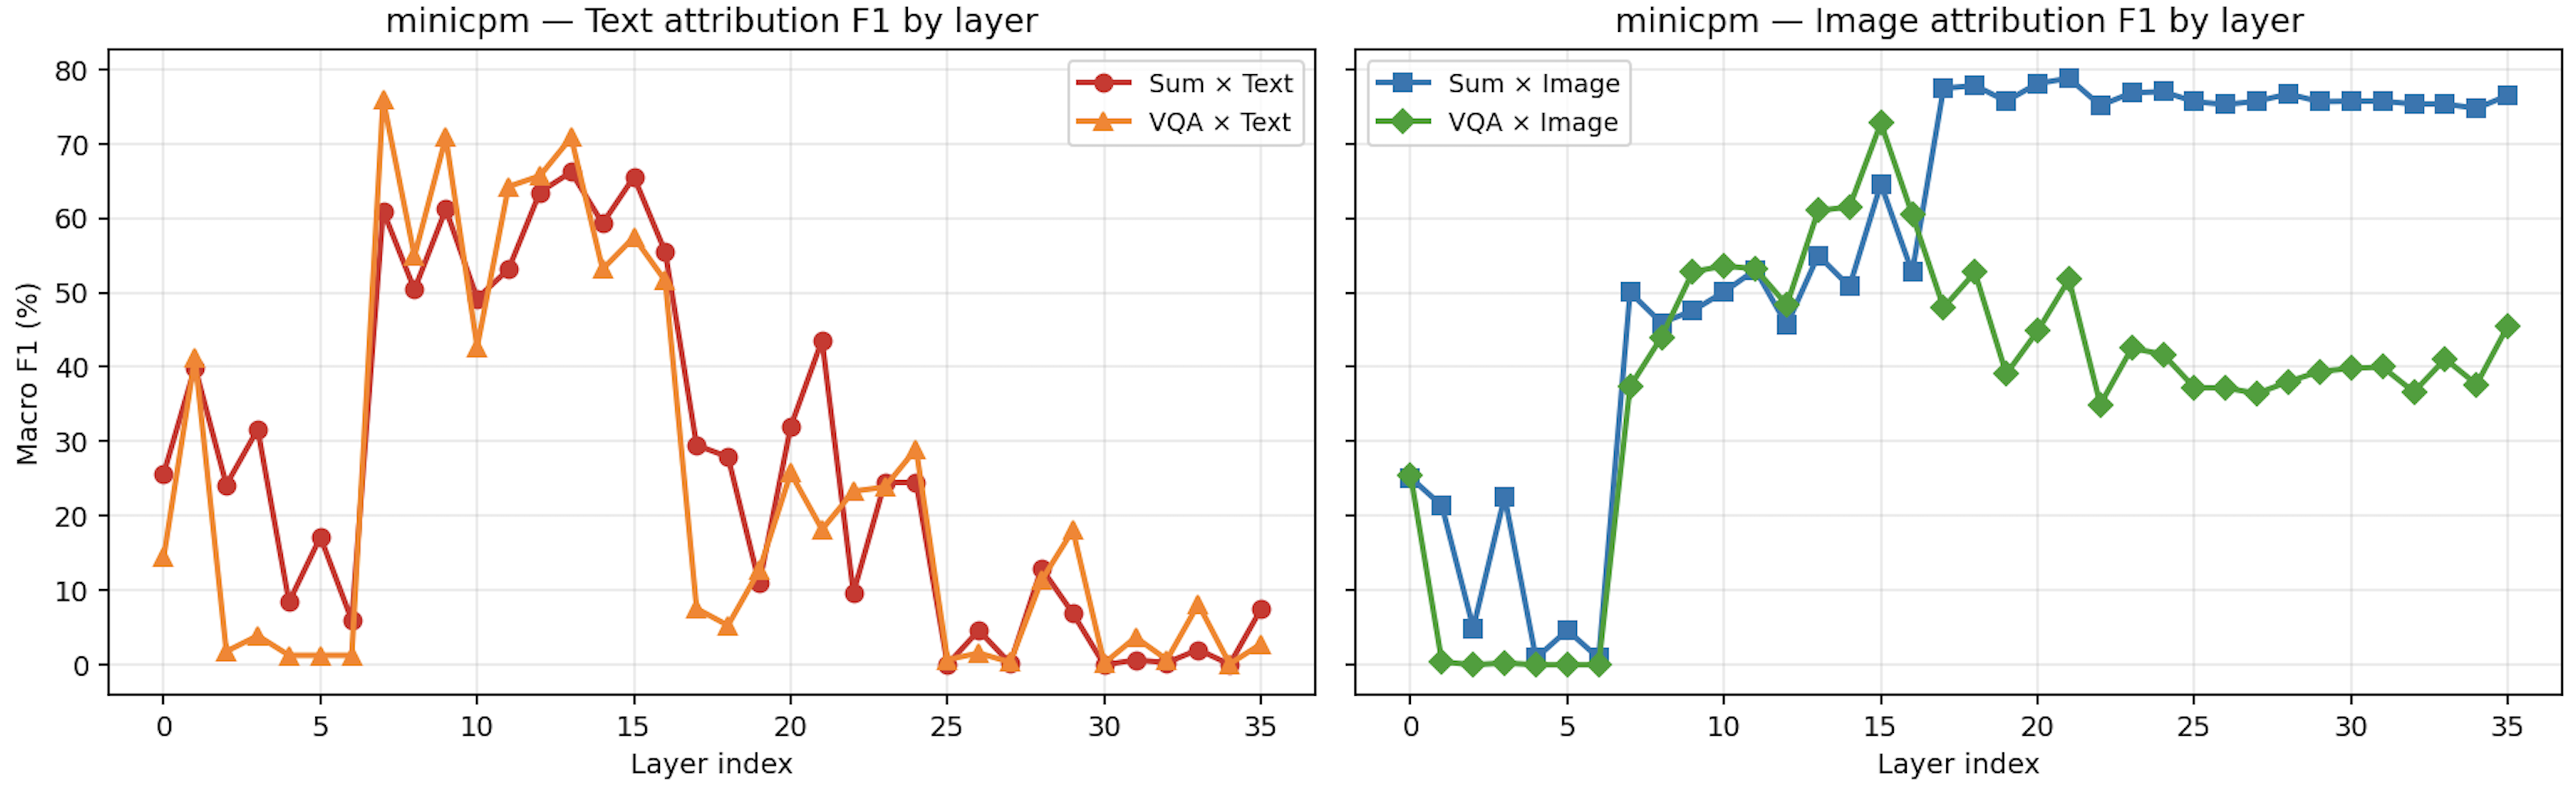
\includegraphics[width=0.92\textwidth]{media/figure/layer.png}
\caption{\textbf{Per-layer attention probe on MiniCPM (36 layers).}
Text (left) and image (right) attribution F1 as a function of the scoring layer.
Three regimes emerge: noisy early layers (L$\le$6), a balanced mid-band (L7--16) that carries both text and image signal, and image-specialized late layers (L$\ge$17) that abandon text grounding.
Averaging across all layers (\texttt{attmean}) dilutes the mid-band text signal with many near-zero layers.}
\label{fig:layer_probe}
\end{figure*}

\subsection{Source Curation Ablation (Visual)}
\Cref{tab:ablation_filtering} reports the visual curation ablation referenced in \Cref{sec:problem} and in the main results; the full per-component analysis on visual, audio, and video tasks is in Appendix~\ref{appendix:ablation_filtering}.

% NOTE: if you prefer this table adjacent to the audio/video ablation (Table in
% Appendix A.2), move the \input line below into sec/appendix/curate_source.tex.
\begin{table}[t]
\centering
\tablesize
\caption{
Ablation study of the source curation framework. 
We report Precision, Recall, and F1 for text and image attribution on the 257 visual summarization task.
The full model integrates POS-aware weighting, confidence shaping, and run-level coherence.
Full ablation results and analysis on audio and video QA tasks can be found in Appendix~\ref{appendix:ablation_filtering_audio_video}.
}
\label{tab:ablation_filtering}
\skiptablebegin
\setlength{\tabcolsep}{4pt}
\begin{tabular}{l|ccc|ccc}
\toprule
\multirow{2}{*}{\textbf{Method}} 
& \multicolumn{3}{c|}{\textbf{Text Attribution}} 
& \multicolumn{3}{c}{\textbf{Image Attribution}} \\
\cmidrule(lr){2-4} \cmidrule(lr){5-7}
& Precision & Recall & F1 
& Precision & Recall & F1 \\
\midrule
Full Model (Default) & 83.06 & 75.10 & 75.66 & 84.19 & 75.12 & 76.59 \\
\midrule
w/o POS Weighting & 82.80 & 77.13 & 76.69 & 23.70 & 19.94 & 20.79 \\
w/o Confidence Weight & 76.82 & 78.82 & 74.59 & 22.88 & 18.85 & 19.88 \\
w/o Confidence & 68.13 & 80.96 & 70.85 & 22.84 & 18.94 & 19.91 \\
w/o Run Coherence & 83.09 & 75.52 & 75.93 & 22.88 & 18.85 & 19.88 \\
w/o $p_{\min}$ Filtering & 82.92 & 75.70 & 76.00 & 22.88 & 18.85 & 19.88 \\
\bottomrule
\end{tabular}
\skiptableend
\end{table}

\subsection{Human--Judge Agreement (Per Slice)}
\Cref{tab:human} gives the per-slice ranking agreement summarized in the experimental setup (mean Kendall $\tau=0.881$, $94.0\%$ concordance).

% Kendall tau / pairwise concordance table — Human vs LLM-judge label rankings
 
\begin{table}[h!]
\label{tab:human}
\centering
\vspace{-5pt}
\renewcommand{\arraystretch}{1.05}
\setlength{\tabcolsep}{4pt}
\scriptsize
\begin{tabular}{l|cc}
\hline
Slice & Kendall $\tau$ & Pairwise concordance \\
\hline
Sum $\times$ Text  & 0.857          & 26/28 (92.9\%) \\
Sum $\times$ Image & \textbf{0.929} & 27/28 (96.4\%) \\
VQA $\times$ Image & 0.857          & 26/28 (92.9\%) \\
\hline
\textbf{Mean} & \textbf{0.881} & \textbf{94.0\%} \\
\hline
\end{tabular}
\vspace{-8pt}
\caption{\scriptsize Ranking consistency between human and LLM-judge labels (Qwen2.5-Omni). Rankings are highly stable across label sources.}
\vspace{-5pt}
\end{table}

\subsection{ASR Segmentation and Modality Availability}
\label{appendix:modality_ablation}
\Cref{fig:ablation_asr} reports the two temporal-attribution factors summarized in the main text.

\begin{figure*}[t]
\setlength\tabcolsep{0pt}
\setlength{\abovecaptionskip}{0.1cm}
\centering
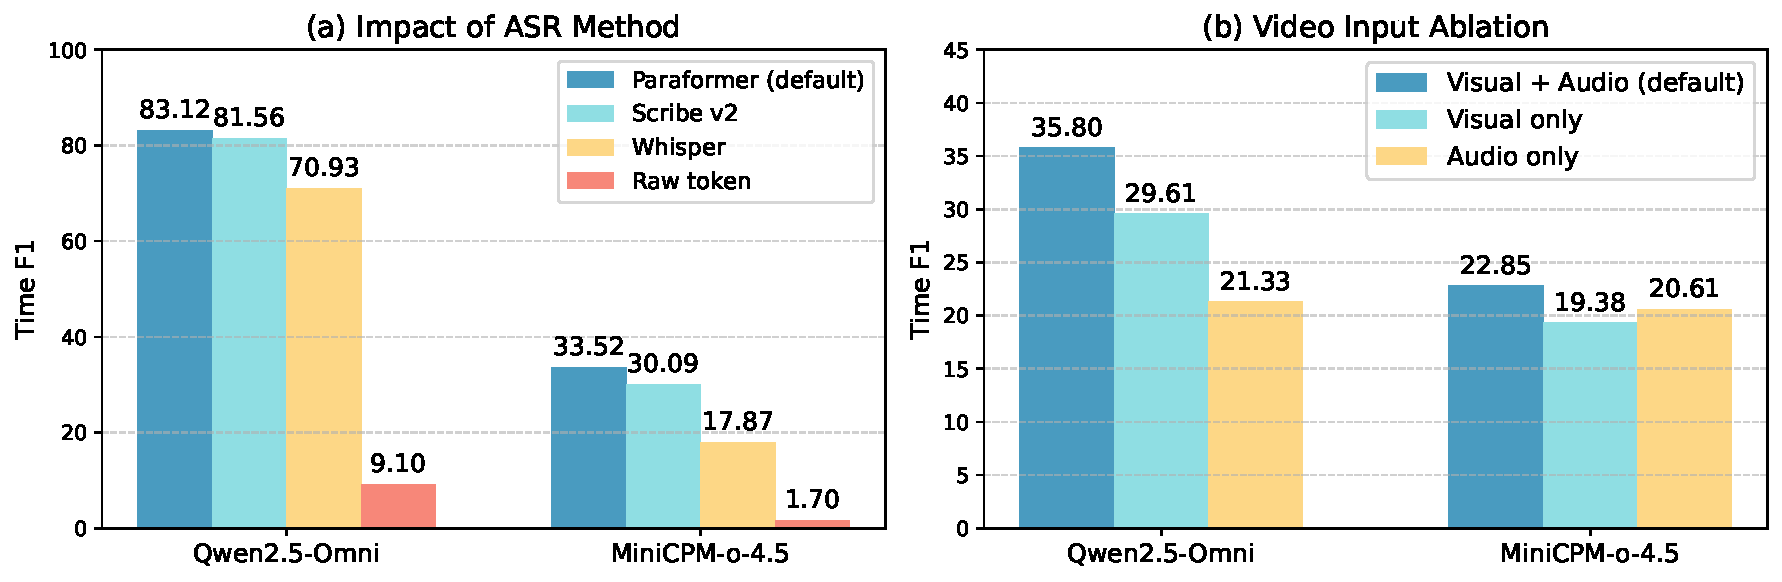
\includegraphics[width=0.92\textwidth]{media/figure/ablation_asr_video.pdf}
\caption{\textbf{Effect of input modality segmentation and availability on attribution performance.}
(a) Impact of ASR segmentation quality on audio attribution. Time-F1 on audio summarization using different ASR systems: high-quality ASR segmentation (Paraformer, Scribe v2) substantially improves accuracy, while raw token inputs without semantic segmentation degrade severely.
(b) Video input ablation. Using both visual and audio signals (default) consistently beats either modality alone, indicating that video attribution benefits from jointly leveraging complementary visual and auditory evidence.}
\label{fig:ablation_asr}
\end{figure*}

\paragraph{ASR segmentation is critical.}
Audio attribution requires mapping generated spans to temporally localized speech segments. We compare three ASR systems of varying quality---Paraformer~\cite{gao2022paraformer}, Scribe v2, and Whisper~\cite{radford2023robust}---against a raw token baseline without ASR segmentation (\Cref{fig:ablation_asr}(a); ASR details in Appendix~\ref{appendix:asr_model}). High-quality ASR dramatically improves performance: Paraformer achieves 83.12 Time-F1 on Qwen and 33.52 on MiniCPM, with Scribe v2 comparable, while removing semantic segmentation (raw tokens) causes severe degradation. Qwen consistently outperforms MiniCPM across all ASR conditions, but both exhibit the same sensitivity to segmentation quality, indicating that the dependence on structured temporal units is not specific to a particular architecture.

\paragraph{Complementary modalities improve video attribution.}
Video inputs contain both visual frames and audio tracks; in OmniTrace, attribution is computed jointly over both, and the final source set is the union of curated visual and audio sources. \Cref{fig:ablation_asr}(b) reports Time-F1 on video QA under three settings. For Qwen2.5-Omni, the full multimodal setting achieves 35.80 Time-F1, versus 29.61 (visual only) and 21.33 (audio only). For MiniCPM-o-4.5, visual-only attribution performs slightly worse than multimodal while audio-only remains competitive with visual-only, suggesting that different MLLMs rely on modality signals differently, but combining modalities still produces the most reliable attribution overall.

\subsection{Positional and Modality Attribution Bias}
\label{appendix:bias}
We analyze whether attribution produced by OmniTrace exhibits systematic biases with respect to input position or modality. \Cref{fig:ablation_bias} summarizes the results.

\begin{figure*}[t]
\setlength\tabcolsep{0pt}
\setlength{\abovecaptionskip}{0.1cm}
\centering
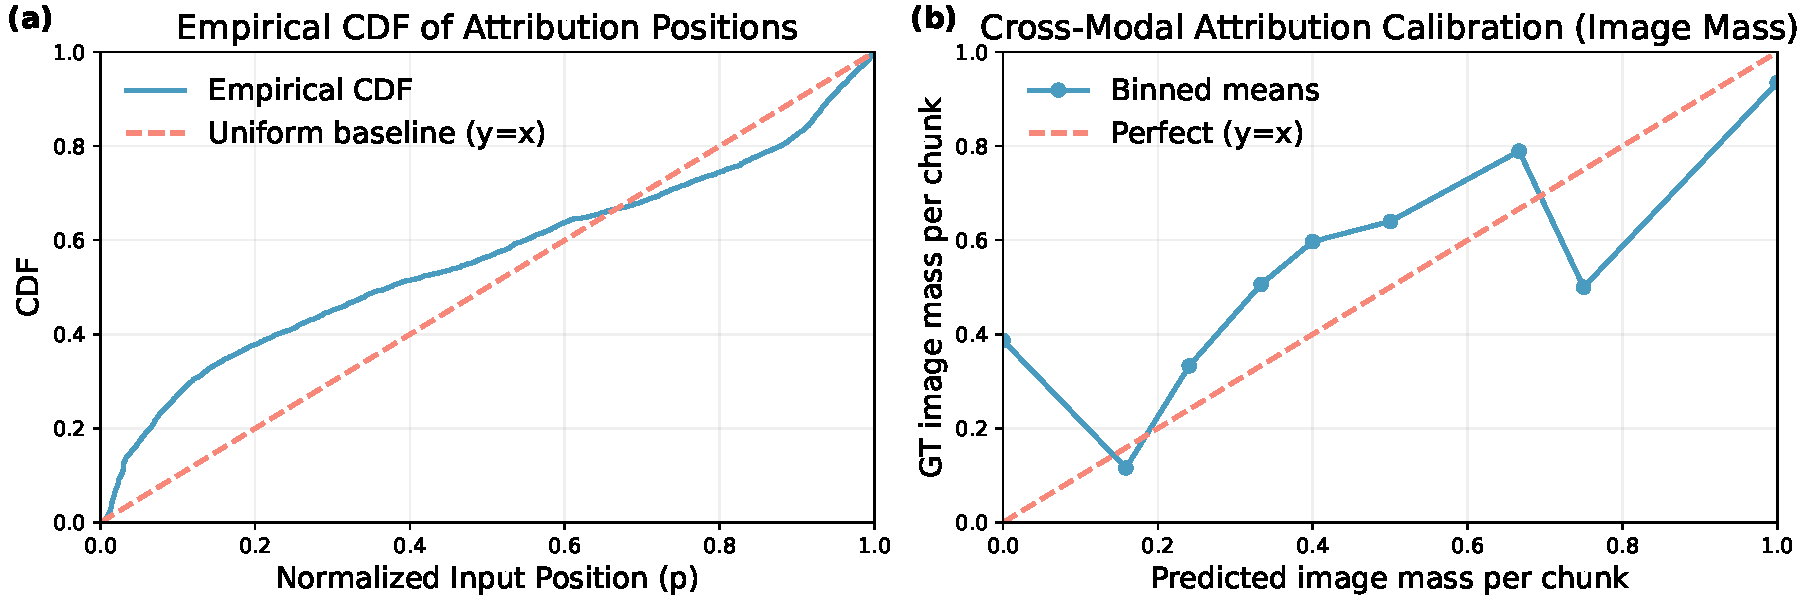
\includegraphics[width=0.92\textwidth]{media/figure/ablation_bias.pdf}
\caption{\textbf{Positional and cross-modal attribution behavior.}
(a) Empirical CDF of normalized attribution positions; the curve above the diagonal indicates early-position bias.
(b) Cross-modal calibration between predicted and ground-truth image mass; deviations from the diagonal reflect regime-dependent calibration effects rather than a strong global modality bias.}
\label{fig:ablation_bias}
\end{figure*}

\paragraph{Positional attribution bias.}
To examine whether attribution is uniformly distributed across the input in summarization tasks, we analyze the normalized position $p \in [0,1]$ of selected source units. \Cref{fig:ablation_bias}(a) shows the empirical CDF of attribution positions. If attribution were position-neutral, the curve would follow the uniform diagonal; instead it lies consistently above the baseline, indicating an early-token bias, with mean normalized position $\bar{p}=0.44 < 0.5$. This appears even in summarization, where evidence may originate anywhere in the input, suggesting that decoder-only omni-modal models preferentially ground generation in earlier context, possibly reflecting attention dynamics or positional priors. A related but far more extreme manifestation appears in \Cref{sec:permodel}, where MiniCPM concentrates $97\%$ of its text attribution on the earliest chunk; the distinction matters, as the effect here is a mild, distributed preference whereas MiniCPM's is a degenerate attention-sink artifact that the per-layer probe corrects.

\paragraph{Cross-modal attribution bias.}
We next analyze whether attribution favors one modality when both visual and textual evidence are available. \Cref{fig:ablation_bias}(b) shows calibration between predicted and ground-truth image attribution mass. Rather than following the diagonal, we observe a non-linear pattern: in the moderate regime (predicted image mass between $0.3$ and $0.6$) the curve lies slightly above the diagonal (mild under-attribution to image evidence in mixed-modality chunks), while at high predicted image mass (above $0.7$) it falls below (occasional overconfidence in image-dominant explanations). Crucially, the curve does not lie uniformly above or below the diagonal, so these are localized calibration effects rather than a systematic global preference for either modality.

\subsection{Generation Quality vs Attribution Quality}
\label{appendix:gen_vs_attr}
We analyze whether attribution quality correlates with generation quality. For QA tasks, generation quality is measured by answer correctness; for summarization, by ROUGE-L.

\begin{figure*}[t]
\setlength\tabcolsep{0pt}
\setlength{\abovecaptionskip}{0.1cm}
\centering
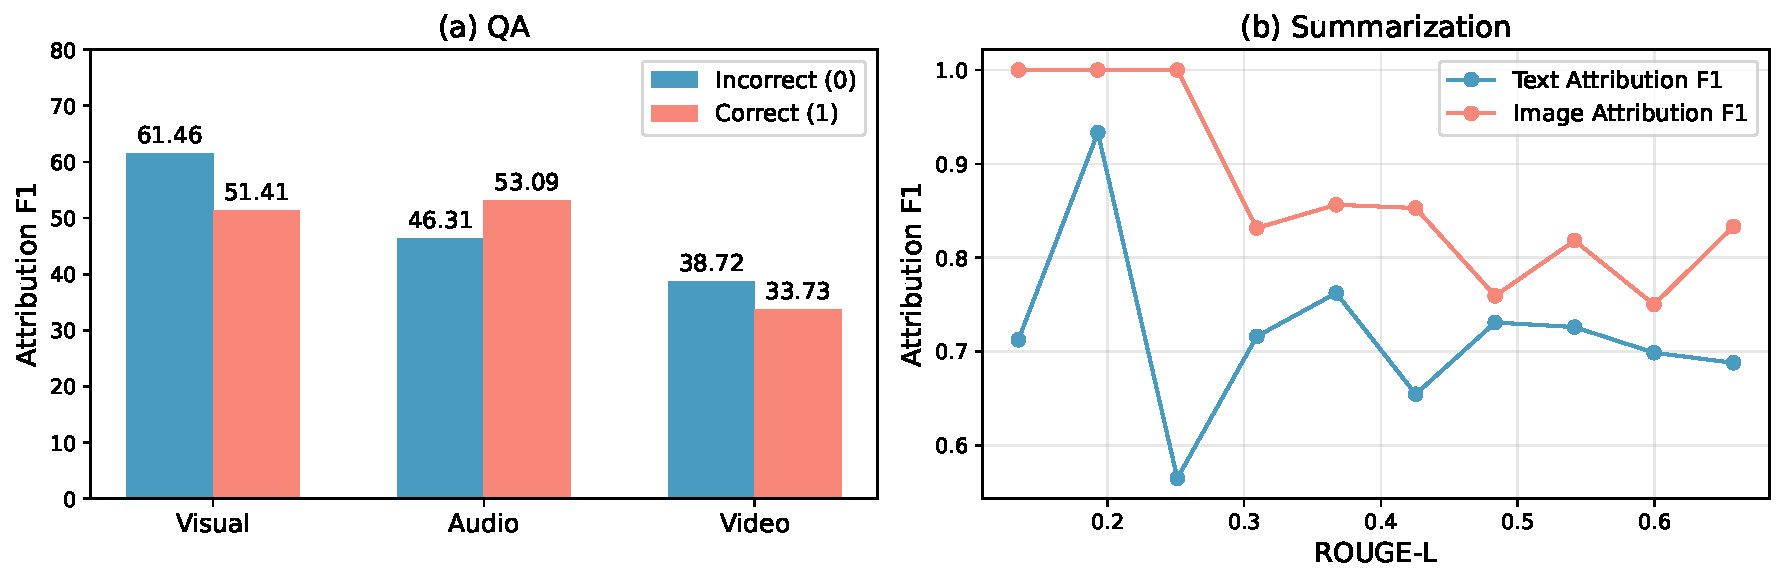
\includegraphics[width=0.92\textwidth]{media/figure/generation_vs_attribution.pdf}
\caption{\textbf{Relationship between generation quality and attribution quality.}
(a) Attribution F1 for QA tasks, grouped by whether the generated answer is correct.
(b) Attribution performance on visual summarization as a function of ROUGE-L.
Attribution quality generally improves with generation quality in some modalities (e.g., audio) but not strictly monotonically, indicating that attribution reflects grounding behavior rather than merely output correctness.}
\label{fig:gen_vs_attr}
\end{figure*}

\paragraph{QA: correctness.}
\Cref{fig:gen_vs_attr}(a) shows attribution F1 for correct versus incorrect answers. Attribution quality does not always increase when answers are correct: in visual and video QA, scores remain comparable or even slightly higher for incorrect predictions, suggesting that the model may still attend to relevant evidence even when its final answer is wrong. In contrast, audio QA shows improved attribution for correct responses, indicating that accurate temporal grounding may contribute more directly to answer correctness.

\paragraph{Summarization: ROUGE-L.}
\Cref{fig:gen_vs_attr}(b) examines summarization using ROUGE-L as a proxy for generation quality. We observe a weak positive correlation between ROUGE-L and attribution F1, particularly for text attribution, but the relationship remains noisy and non-monotonic, indicating that attribution quality is not simply a byproduct of better generation. Overall, attribution captures aspects of the model's evidence-grounding behavior that are partially independent of final output quality.